\section{Empirical Failure Modes of OPD}
\label{sec:failure-modes}

We first identify pathological OPD training dynamics: sample inefficiency, unstable generation behavior, and a persistent gap to full-vocabulary OPD (\secref{subsec:training-dynamics}). We then trace them to high-variance log-ratio rewards, whose extremes concentrate early and persist throughout training (\secref{subsec:high-variance}). Finally, we show that standard RL reward-stabilization strategies fail to fix these pathologies (\secref{subsec:standard-fixes}).

\subsection{Pathological Training Dynamics}
\label{subsec:training-dynamics}

We begin by empirically examining the training dynamics of OPD. We train a Qwen3-1.7B student with a Qwen3-4B teacher and monitor performance on \textsc{MATH-500}  \citep{hendrycks2021math}. As shown in \autoref{fig:standard-fixes}, OPD exhibits three pathological behaviors. \emph{(i) OPD is sample-inefficient.} Accuracy initially decreases and does not begin to recover until roughly 300 training steps, despite the availability of dense token-level supervision. \emph{(ii) OPD is unstable in both accuracy and generation behavior.} Validation accuracy fluctuates substantially, while the average validation response length undergoes large oscillations and stabilizes only after around 400 steps, suggesting that the student policy moves through unstable generation regimes during training. \emph{(iii) OPD converges to a substantially weaker policy than full-vocabulary OPD.}
Full-vocabulary OPD computes the distillation signal over the entire vocabulary rather than only the sampled student token \citep{zhao2026decouplingkltrajectoriesunified}. On \textsc{MATH-500}, OPD plateaus at 54.93\%, whereas full-vocabulary OPD reaches 63.12\%, leaving an 8.19-point gap and recovering only 69.44\% of the teacher's validation accuracy.



\subsection{Pathological Reward Distributions}
\label{subsec:high-variance}

To understand what undermines OPD training, we examine its dense token-level rewards. Since these rewards directly scale the policy-gradient updates, their distribution determines how stable and reliable the optimization signal is.

\paragraph{OPD rewards exhibit extremely high variance.}
We examine the reward distribution induced by OPD before training. Using the Qwen3-1.7B-Base student and the Qwen3-4B teacher, we sample 512 examples from \textsc{MATH-500}, generate student rollouts, and compute the OPD reward \(r_t^{\mathrm{OPD}}(c_t,o_t)\) for every rollout token. We collect these token-level rewards across all rollouts and plot their empirical distribution. As shown in \autoref{fig:reward-diagnosis}(a), OPD rewards span an extremely wide range, with the negative tail reaching nearly \(-50\). This high-variance distribution is a direct consequence of the log difference, which can amplify teacher--student probability discrepancies into unbounded reward magnitudes \citep{ko2026reopold, jia2026asymmetric}. Because each policy-gradient update is directly scaled by this reward scalar, extreme OPD rewards artificially inflate gradient variance and make optimization fragile.

\begin{figure}[t]
  \centering
  \begin{minipage}[t]{0.49\columnwidth}
    \centering
    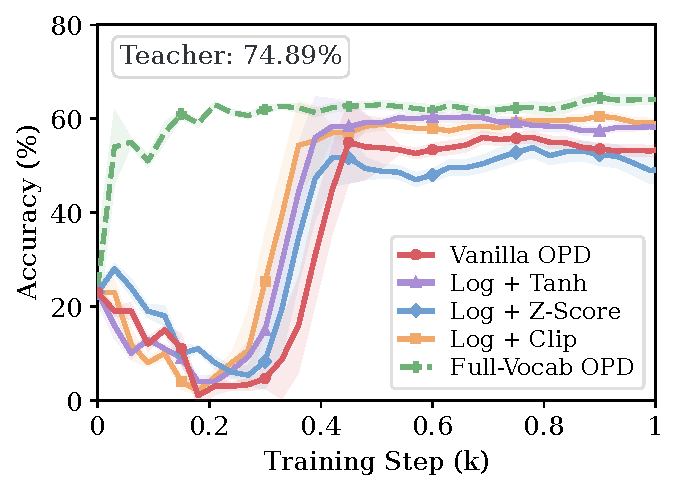
\includegraphics[width=\linewidth]{figures/fig2a_log_training_4b.pdf}\\[-0.5ex]
    \textbf{(a)}
  \end{minipage}\hfill
  \begin{minipage}[t]{0.49\columnwidth}
    \centering
    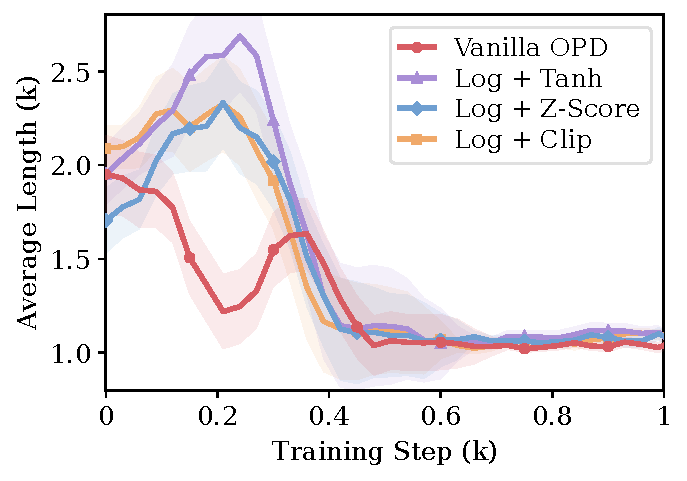
\includegraphics[width=\linewidth]{figures/fig2b_log_training_8b.pdf}\\[-0.5ex]
    \textbf{(b)}
  \end{minipage}
  \vspace{-7pt}
    \caption{
    Pathological OPD training dynamics. 
    OPD shows (a) delayed, unstable accuracy far below full-vocabulary OPD and (b) response-length oscillations.
    }
    \vspace{-15pt}
  \label{fig:standard-fixes}
\end{figure}

\paragraph{Extreme rewards concentrate at early rollout positions.}
We group OPD rewards by rollout token index and compute position-wise mean, minimum, and maximum values, filtering positions with too few samples. As shown in \autoref{fig:reward-diagnosis}(b), the most extreme rewards occur near the beginning of student rollouts. This pattern is especially harmful in on-policy training: unstable rewards on early tokens can shift the prefix distribution, and subsequent rollouts then condition on these shifted prefixes, propagating instability to later tokens \citep{ liu2026prefixteachsuffixfade}. This feedback loop destabilizes the training distribution and contributes to fluctuations in both validation accuracy and response length.
\paragraph{Extreme rewards persist across training.}
We track the reward dynamics during OPD training by recording batch-level statistics over all rollout-token rewards at each training step, including the minimum, maximum, and the \(5\)th--\(95\)th percentile range. As shown in \autoref{fig:reward-diagnosis}(c), extreme positive and negative rewards persist throughout training and remain close to their initial scale. This indicates that high-variance rewards are not merely an initialization artifact or an early-stage transient. Instead, OPD is exposed to severe token-level rewards and penalties throughout optimization.

\subsection{Post-Hoc Reward Stabilization Fails}
\label{subsec:standard-fixes}

\begin{table}[t]
  \centering
  \small
  \begin{tabular}{lll}
    \toprule
    \textbf{Method} & \textbf{Transformation} & \textbf{Effect} \\
    \midrule
    \emph{Clip} 
      & $\mathrm{clip}(r_t^{\mathrm{OPD}}, c_l, c_h)$ 
      & Hard truncation \\
    \emph{Tanh} 
      & $\tanh(r_t^{\mathrm{OPD}} / \tau)$ 
      & Smooth compression \\
    \emph{Z-Score} 
      & $(r_t^{\mathrm{OPD}} - \mu_B) / \sigma_B$ 
      & Batch normalization \\
    \bottomrule
  \end{tabular}
  \vspace{-7pt}
    \caption{Post-hoc OPD reward transformations.}
    \vspace{-15pt}
  \label{tab:standard-fixes}
\end{table}

\begin{table*}[t]
\centering

\begin{subtable}{\linewidth}
\centering
\scriptsize
\setlength{\tabcolsep}{1.0pt}
\renewcommand{\arraystretch}{1.05}
\caption{Teacher: Qwen3-4B $\to$ Student: Qwen3-0.6B-Base}
\label{tab:main-4b}
\begin{adjustbox}{max width=\linewidth}
\begin{tabular}{@{}ll lll@{\hskip 6pt}lll@{\hskip 6pt}lll@{\hskip 6pt}lll@{\hskip 6pt}lll@{\hskip 6pt}lll@{\hskip 6pt}lll@{\hskip 6pt}lll@{}}
\toprule
 &  & \multicolumn{3}{c}{GSM8K} & \multicolumn{3}{c}{MATH500} & \multicolumn{3}{c}{AMC23} & \multicolumn{3}{c}{AIME24} & \multicolumn{3}{c}{AIME25} & \multicolumn{3}{c}{Minerva} & \multicolumn{3}{c}{Olympiad} & \multicolumn{3}{c}{Mean} \\
Class & Param & Avg & Pass & Len & Avg & Pass & Len & Avg & Pass & Len & Avg & Pass & Len & Avg & Pass & Len & Avg & Pass & Len & Avg & Pass & Len & Avg & Pass & Len \\
\cmidrule(lr){3-5} \cmidrule(lr){6-8} \cmidrule(lr){9-11} \cmidrule(lr){12-14} \cmidrule(lr){15-17} \cmidrule(lr){18-20} \cmidrule(lr){21-23} \cmidrule(lr){24-26}
\midrule
\multirow{1}{*}{Full-vocab} & -- & 66.04 & 87.08 & 4087 & 43.90 & 54.84 & 4096 & 28.75 & 40.00 & 4096 & \textbf{3.33} & \textbf{10.00} & 4096 & 1.67 & 3.33 & 4096 & 11.03 & 15.81 & 4077 & 5.62 & 25.00 & 4094 & 22.91 & 33.72 & 4092 \\
\cmidrule(lr){1-26}
\multirow{4}{*}{Vanilla} & -- & 61.50 & 86.81 & 4078 & 36.02 & 61.20 & 4084 & 14.37 & 47.50 & 4096 & 1.67 & \underline{6.67} & 4096 & 0.83 & 3.33 & 4085 & 6.99 & 17.65 & 4065 & 12.50 & 30.07 & 4087 & 19.13 & 36.18 & 4084 \\
 & + Clip & 65.90 & 87.26 & 498 & 42.27 & 63.24 & 1483 & 21.88 & 52.50 & 2669 & 0.42 & 3.33 & 3722 & 1.25 & 6.67 & 3842 & 10.06 & 21.69 & 1378 & 15.67 & 33.78 & 2809 & 22.49 & 38.35 & 2343 \\
 & + Tanh & 65.38 & 87.00 & 502 & 43.88 & 62.00 & 1493 & 22.69 & 52.50 & 2609 & 0.42 & 3.33 & 3786 & 0.42 & 3.33 & 3880 & 10.03 & 23.00 & 1329 & 4.62 & 15.00 & 3872 & 21.06 & 35.17 & 2496 \\
 & + Z-Score & 56.21 & 86.43 & 437 & 35.75 & 62.26 & 1571 & 14.37 & 45.00 & 2648 & 0.42 & 3.33 & 3691 & 0.42 & 3.33 & 3703 & 8.00 & 20.22 & 1410 & 12.61 & 31.41 & 2750 & 18.25 & 36.00 & 2316 \\
\cmidrule(lr){1-26}
\multirow{8}{*}{PowerOPD} & $\alpha=0.1$ & 68.58 & \underline{89.23} & 404 & 43.62 & 64.92 & 1482 & 28.12 & \underline{57.50} & 2558 & 2.50 & \underline{6.67} & 3623 & 0.42 & 3.33 & 3806 & 9.38 & 20.96 & 1391 & 16.48 & 34.67 & 2776 & \cellcolor{avgshade!12}24.16 & \cellcolor{passshade!12}39.61 & \cellcolor{lenshade!12}2291 \\
 & $\alpha=0.5$ & 68.67 & \underline{89.23} & 407 & 45.29 & \textbf{66.92} & 1438 & 26.88 & 55.00 & 2617 & 2.50 & \underline{6.67} & 3633 & 1.25 & 6.67 & 3662 & 10.62 & 23.16 & 1225 & 16.96 & \underline{36.15} & 2704 & \cellcolor{avgshade!33}24.60 & \cellcolor{passshade!38}40.54 & \cellcolor{lenshade!30}2241 \\
 & $\alpha=1$ & \underline{69.48} & \textbf{90.22} & 396 & 44.34 & 66.18 & 1451 & 24.38 & 47.50 & 2628 & 2.08 & 3.33 & 3583 & \underline{2.50} & \underline{10.00} & 3703 & 10.57 & \textbf{24.26} & 1236 & \textbf{17.22} & 35.85 & 2701 & \cellcolor{avgshade!22}24.37 & \cellcolor{passshade!12}39.62 & \cellcolor{lenshade!21}2243 \\
 & $\alpha=5$ & 69.19 & 88.55 & \textbf{374} & \textbf{45.66} & \underline{66.38} & 1417 & \textbf{31.12} & \underline{57.50} & 2456 & 2.50 & 3.33 & 3610 & 0.83 & 6.67 & 3629 & \textbf{12.22} & 23.63 & \underline{1129} & 16.87 & 35.85 & 2677 & \cellcolor{avgshade!74}\underline{25.48} & \cellcolor{passshade!30}40.27 & \cellcolor{lenshade!39}2185 \\
 & $\alpha=10$ & 69.42 & 88.55 & 393 & \underline{45.54} & 65.92 & 1388 & \underline{29.69} & \underline{57.50} & 2426 & 2.08 & 3.33 & 3597 & 1.25 & 3.33 & 3612 & 11.31 & \underline{23.90} & \textbf{1124} & 17.11 & 35.26 & 2664 & \cellcolor{avgshade!61}25.20 & \cellcolor{passshade!14}39.68 & \cellcolor{lenshade!48}2172 \\
 & $\alpha=50$ & 69.25 & 87.11 & \underline{385} & 45.12 & 66.00 & 1367 & 24.69 & \textbf{60.00} & 2358 & \underline{2.92} & \textbf{10.00} & 3283 & 0.83 & 6.67 & 3502 & 11.31 & 22.43 & 1149 & \underline{17.20} & \textbf{36.59} & 2571 & \cellcolor{avgshade!27}24.47 & \cellcolor{passshade!58}\underline{41.26} & \cellcolor{lenshade!57}2088 \\
 & $\alpha=100$ & 68.70 & 86.88 & \underline{385} & 44.57 & 65.66 & \underline{1363} & 28.12 & 57.00 & \underline{2230} & 2.50 & \textbf{10.00} & \underline{3282} & 0.83 & 6.67 & \underline{3324} & 10.75 & 23.69 & 1225 & 17.04 & \underline{36.15} & \underline{2490} & \cellcolor{avgshade!35}24.64 & \cellcolor{passshade!47}40.86 & \cellcolor{lenshade!66}\underline{2043} \\
 & $\alpha=500$ & \textbf{69.77} & 87.49 & 397 & 44.62 & 65.50 & \textbf{1324} & 29.25 & \underline{57.50} & \textbf{2049} & \textbf{3.33} & \textbf{10.00} & \textbf{3077} & \textbf{2.92} & \textbf{13.33} & \textbf{2819} & \underline{11.40} & 23.53 & 1273 & \textbf{17.22} & 35.85 & \textbf{2185} & \cellcolor{avgshade!75}\textbf{25.50} & \cellcolor{passshade!75}\textbf{41.89} & \cellcolor{lenshade!75}\textbf{1875} \\
\bottomrule
\end{tabular}
\end{adjustbox}
\end{subtable}

\vspace{0.5em}

\begin{subtable}{\linewidth}
\centering
\scriptsize
\setlength{\tabcolsep}{1.0pt}
\renewcommand{\arraystretch}{1.05}
\caption{Teacher: Qwen3-8B $\to$ Student: Qwen3-0.6B-Base}
\label{tab:main-8b}
\begin{adjustbox}{max width=\linewidth}
\begin{tabular}{@{}ll lll@{\hskip 6pt}lll@{\hskip 6pt}lll@{\hskip 6pt}lll@{\hskip 6pt}lll@{\hskip 6pt}lll@{\hskip 6pt}lll@{\hskip 6pt}lll@{}}
\toprule
 &  & \multicolumn{3}{c}{GSM8K} & \multicolumn{3}{c}{MATH500} & \multicolumn{3}{c}{AMC23} & \multicolumn{3}{c}{AIME24} & \multicolumn{3}{c}{AIME25} & \multicolumn{3}{c}{Minerva} & \multicolumn{3}{c}{Olympiad} & \multicolumn{3}{c}{Mean} \\
Class & Param & Avg & Pass & Len & Avg & Pass & Len & Avg & Pass & Len & Avg & Pass & Len & Avg & Pass & Len & Avg & Pass & Len & Avg & Pass & Len & Avg & Pass & Len \\
\cmidrule(lr){3-5} \cmidrule(lr){6-8} \cmidrule(lr){9-11} \cmidrule(lr){12-14} \cmidrule(lr){15-17} \cmidrule(lr){18-20} \cmidrule(lr){21-23} \cmidrule(lr){24-26}
\midrule
\multirow{1}{*}{Full-vocab} & -- & \textbf{70.85} & 88.48 & 4095 & \textbf{46.53} & 54.38 & 4095 & 27.50 & 35.00 & 4096 & \textbf{5.00} & 6.67 & 4096 & \textbf{3.33} & 6.67 & 4096 & \underline{11.58} & 15.07 & 4089 & 6.62 & 21.00 & 4096 & 24.49 & 32.47 & 4095 \\
\cmidrule(lr){1-26}
\multirow{4}{*}{Vanilla} & -- & 60.59 & 86.35 & 416 & 40.43 & 64.00 & 1450 & 22.19 & 50.00 & 2393 & 0.83 & 3.33 & 3436 & 0.83 & 6.67 & 3752 & 9.01 & 20.59 & 1306 & 14.35 & 33.33 & 2708 & 21.18 & 37.75 & 2209 \\
 & + Clip & 67.99 & 87.64 & 398 & 43.75 & 65.30 & 1429 & \underline{28.12} & 52.50 & 2538 & 1.67 & 6.67 & 3506 & 1.67 & \underline{10.00} & 3711 & 9.42 & 22.06 & 1286 & 16.20 & 34.22 & 2674 & 24.12 & 39.77 & 2220 \\
 & + Tanh & 66.98 & 88.63 & 394 & 43.39 & 64.86 & 1425 & 25.00 & \underline{57.50} & 2468 & 2.92 & \underline{10.00} & 3518 & 1.67 & 6.67 & 3639 & 9.65 & 21.32 & 1281 & 16.89 & 34.52 & 2698 & 23.79 & 40.50 & 2203 \\
 & + Z-Score & 63.83 & 88.10 & 391 & 42.72 & 65.62 & 1364 & 25.62 & 50.00 & 2269 & 1.25 & 6.67 & 3371 & 0.42 & 3.33 & 3578 & 10.71 & 21.32 & 1212 & 15.54 & 35.70 & 2528 & 22.87 & 38.68 & 2102 \\
\cmidrule(lr){1-26}
\multirow{8}{*}{PowerOPD} & $\alpha=0.1$ & 67.18 & 88.02 & 384 & 43.82 & 65.86 & 1395 & 24.06 & 55.00 & 2460 & \underline{3.75} & \textbf{13.33} & 3413 & 0.83 & 6.67 & 3617 & 10.25 & 22.43 & 1195 & 15.94 & 34.67 & 2632 & \cellcolor{avgshade!19}23.69 & \cellcolor{passshade!48}40.85 & \cellcolor{lenshade!21}2157 \\
 & $\alpha=0.5$ & 67.58 & 89.16 & 381 & 45.07 & 66.98 & 1371 & 25.94 & 55.00 & 2535 & 1.67 & 6.67 & 3359 & 0.83 & 6.67 & 3549 & 10.06 & 22.79 & 1144 & \textbf{17.26} & \textbf{36.89} & 2552 & \cellcolor{avgshade!34}24.06 & \cellcolor{passshade!35}40.59 & \cellcolor{lenshade!30}2127 \\
 & $\alpha=1$ & 65.36 & \underline{89.76} & \underline{380} & 44.89 & \textbf{67.10} & 1408 & 23.44 & 52.50 & 2560 & 1.67 & 6.67 & 3584 & 0.83 & 3.33 & 3542 & 11.31 & \textbf{25.37} & 1188 & \underline{17.24} & \underline{36.30} & 2637 & \cellcolor{avgshade!12}23.53 & \cellcolor{passshade!12}40.15 & \cellcolor{lenshade!12}2186 \\
 & $\alpha=5$ & 66.79 & 88.86 & \textbf{364} & 45.33 & 66.72 & 1348 & 25.62 & 55.00 & 2503 & 2.92 & 6.67 & 3512 & \textbf{3.33} & \textbf{13.33} & 3468 & 11.08 & 22.79 & \underline{1076} & 17.13 & 35.11 & 2566 & \cellcolor{avgshade!56}24.60 & \cellcolor{passshade!67}41.21 & \cellcolor{lenshade!39}2120 \\
 & $\alpha=10$ & 66.76 & 87.87 & \textbf{364} & \underline{45.49} & \underline{67.00} & \textbf{1308} & 24.38 & \textbf{60.00} & 2251 & 1.25 & 6.67 & 3274 & 0.83 & 6.67 & 3528 & \textbf{11.76} & \underline{24.63} & \textbf{1056} & \underline{17.24} & 36.00 & 2523 & \cellcolor{avgshade!30}23.96 & \cellcolor{passshade!69}41.26 & \cellcolor{lenshade!48}2043 \\
 & $\alpha=50$ & 69.29 & 88.93 & 382 & 44.91 & 65.78 & \underline{1313} & \underline{28.12} & \underline{57.50} & 2088 & 1.67 & 6.67 & 3262 & 0.42 & 6.67 & 3233 & 11.12 & 23.90 & 1149 & 16.96 & 35.70 & 2449 & \cellcolor{avgshade!58}24.64 & \cellcolor{passshade!42}40.74 & \cellcolor{lenshade!57}1982 \\
 & $\alpha=100$ & 68.63 & \textbf{89.79} & 385 & 45.03 & 65.42 & 1322 & \textbf{29.06} & \underline{57.50} & \underline{2038} & 2.92 & \underline{10.00} & \underline{3164} & 1.25 & \underline{10.00} & \underline{3225} & 11.31 & 22.79 & 1244 & 17.17 & 34.07 & \underline{2331} & \cellcolor{avgshade!75}\textbf{25.05} & \cellcolor{passshade!75}\textbf{41.37} & \cellcolor{lenshade!66}\underline{1958} \\
 & $\alpha=500$ & \underline{70.58} & 87.04 & 427 & 44.59 & 65.42 & 1321 & 22.19 & \underline{57.50} & \textbf{1952} & \textbf{5.00} & 6.67 & \textbf{3059} & \underline{2.08} & \textbf{13.33} & \textbf{2742} & 11.44 & 23.90 & 1309 & 16.83 & 35.26 & \textbf{2201} & \cellcolor{avgshade!59}\underline{24.67} & \cellcolor{passshade!71}\underline{41.30} & \cellcolor{lenshade!75}\textbf{1859} \\
\bottomrule
\end{tabular}
\end{adjustbox}
\end{subtable}

\vspace{-4pt}
\caption{
Mathematical reasoning evaluation with the Qwen3-0.6B student. \textbf{Bold} and \underline{underline} denote the best and second-best results. Color intensity highlights the relative performance of PowerOPD variants across different \(\alpha\). Log reward denotes OPD reward variants without post-hoc stabilization.
Avg, Pass, and Len denote Avg@8, Pass@8, and average response length, respectively.
}
\label{tab:main}
\end{table*}

The high variance of OPD rewards originates from the unboundedness of the log-ratio form. The OPD reward \(r_t^{\mathrm{OPD}}=\log(\pi_T/\pi_\theta)\) diverges in both directions\footnote{Full-vocabulary OPD shares the same unbounded log-ratio, but 
computes an exact expectation where extreme values are suppressed by 
their small probability weights. Sampled-token OPD lacks this 
averaging, exposing the gradient directly to extreme log-ratios.}: \(r_t^{\mathrm{OPD}}\to +\infty\) when \(\pi_\theta(o_t\mid c_t)\to 0\), and \(r_t^{\mathrm{OPD}}\to -\infty\) when \(\pi_T(o_t\mid c_t)\to 0\). Because OPD evaluates rewards on student-sampled tokens, these tokens tend to have high probability under the student, but the teacher may assign low probability to the same student-sampled tokens. The log-ratio reward can therefore easily enter its negative divergent regime, producing the heavy negative tail observed in \autoref{fig:reward-diagnosis}(a).
A standard remedy is to apply post-hoc reward transformations from RL, where clipping and normalization are widely used to stabilize optimization \citep{mnih2015human,andrychowicz2020matters}. We consider three representative methods, summarized in \autoref{tab:standard-fixes}: \emph{Clip} truncates rewards at fixed thresholds,\footnote{We set \(c_l=-c_h\), grid-search multiple threshold values, and use the best-performing setting \(c_l=-1, c_h=1\).} \emph{Tanh} maps rewards smoothly into \([-1,1]\), and \emph{Z-Score} centers and rescales rewards using batch statistics. 
% These methods directly target the extreme magnitudes observed above, but all operate only after the log-ratio reward has already been computed. 

\paragraph{Post-hoc stabilization fails to fix.}
As shown in \autoref{fig:standard-fixes}, post-hoc reward stabilization alleviates neither the optimization delay nor the unstable generation dynamics of OPD. \emph{Tanh} and \emph{Z-Score} reduce the gap to full-vocabulary OPD to some extent, but validation accuracy still improves only after a long delay, and response length continues to exhibit large oscillations. \emph{Z-Score} can even underperform vanilla OPD, likely because batch centering may change the sign of rewards and reverse the intended direction of some updates. In contrast, \emph{Clip} and \emph{Tanh} preserve the reward sign, but they only reshape reward magnitudes after the unbounded log-ratio has been computed, leaving the underlying reward form unchanged. These results indicate that \emph{OPD's pathological training dynamics are driven not by the lack of post-hoc stabilization, but by the unbounded log-ratio reward itself.}



